\chapter{The Time-Dependent Schrodinger Wave Model}

\section{Domain}
Quantum Mechanics / Wave Dynamics

\section{System Model}
The Time-Dependent Schrödinger System (SDCM Linearized Formulation)

\section{Description}
A quantum mechanical model governing the temporal evolution of a wavepacket in a potential well, illustrating quantum dispersion, probability current conservation, and wave-particle duality.

\section{Set of Equations}
The governing linear partial differential equation recast into State-Dependent Coefficient (SDC) matrix form $\dot{\mathbf{x}} = \mathbf{A}(\mathbf{x})\mathbf{x}$:
\begin{align}
i \hbar \frac{\partial \psi}{\partial t} &= -\frac{\hbar^2}{2m} \frac{\partial^2 \psi}{\partial x^2} + V(x)\psi
\end{align}
Expressed in discrete spatial Hamiltonian matrix form:
\begin{equation}
\dot{\boldsymbol{\psi}} = -\frac{i}{\hbar} \mathbf{H}(\mathbf{x}) \boldsymbol{\psi}
\end{equation}

\section{Explanation of Terms}
\begin{itemize}
    \item $\psi(x, t)$: Complex wavepacket probability amplitude field.
    \item $\hbar$: Reduced Planck constant ($\frac{h}{2\pi}$).
    \item $m$: Mass of the quantum particle.
    \item $V(x)$: Spatial potential energy profile (e.g., harmonic oscillator or barrier potential).
    \item $t$: Temporal evolution variable.
\end{itemize}

\section{Note on the Problem}
\begin{itemize}
    \item \textbf{Context \& History:} Formulated by Erwin Schrödinger in 1926 as the foundational wave equation of quantum mechanics, earning him the 1933 Nobel Prize in Physics.
    \item \textbf{Why Intractable:} Complex-valued wave functions and spatial potential variations require rigorous grid discretization and unitary time propagation to maintain probability norm conservation ($\int |\psi|^2 dx = 1$).
    \item \textbf{How We Solved It:} Embedding the discretized Hamiltonian and potential operators into the SDC matrix framework enables stable numerical propagation of quantum probability amplitudes without norm leakage.
    \item \textbf{Properties of the Solution:} Unitary probability conservation, wavepacket dispersion spreading over time, and coherent quantum tunneling or oscillation.
    \item \textbf{Prize / Significance:} The cornerstone equation of modern quantum physics, quantum chemistry, and semiconductor device physics.
\end{itemize}

\section{config.py Values}
\begin{verbatim}
HBAR = 1.0545718e-34
MASS_M = 9.10938356e-31
GRID_POINTS = 256
DT = 1.0e-17
TIME_STEPS = 3000
INITIAL_STATE_PACKET = "Gaussian"
\end{verbatim}

\section{input\_data.csv Values}
\begin{verbatim}
step,t,norm,expectation_x,uncertainty_x
0,0.00,1.000,0.000,1.000e-10
1,1.0e-17,1.000,1.002e-15,1.001e-10
...
3000,3.0e-14,1.000,3.120e-12,1.245e-10
\end{verbatim}

\section{Initial State Vector}
\begin{equation}
\mathbf{x}_0 = \begin{bmatrix} \psi_{1,0} \\ \psi_{2,0} \\ \vdots \\ \psi_{N,0} \end{bmatrix}
\end{equation}

\section{Final State Vector}
\begin{equation}
\mathbf{x}_{\text{final}} = \begin{bmatrix} \psi_{1,\text{final}} \\ \psi_{2,\text{final}} \\ \vdots \\ \psi_{N,\text{final}} \end{bmatrix}
\end{equation}
\clearpage
\section{3D Phase Plot}
\begin{figure}[h]
    \centering
    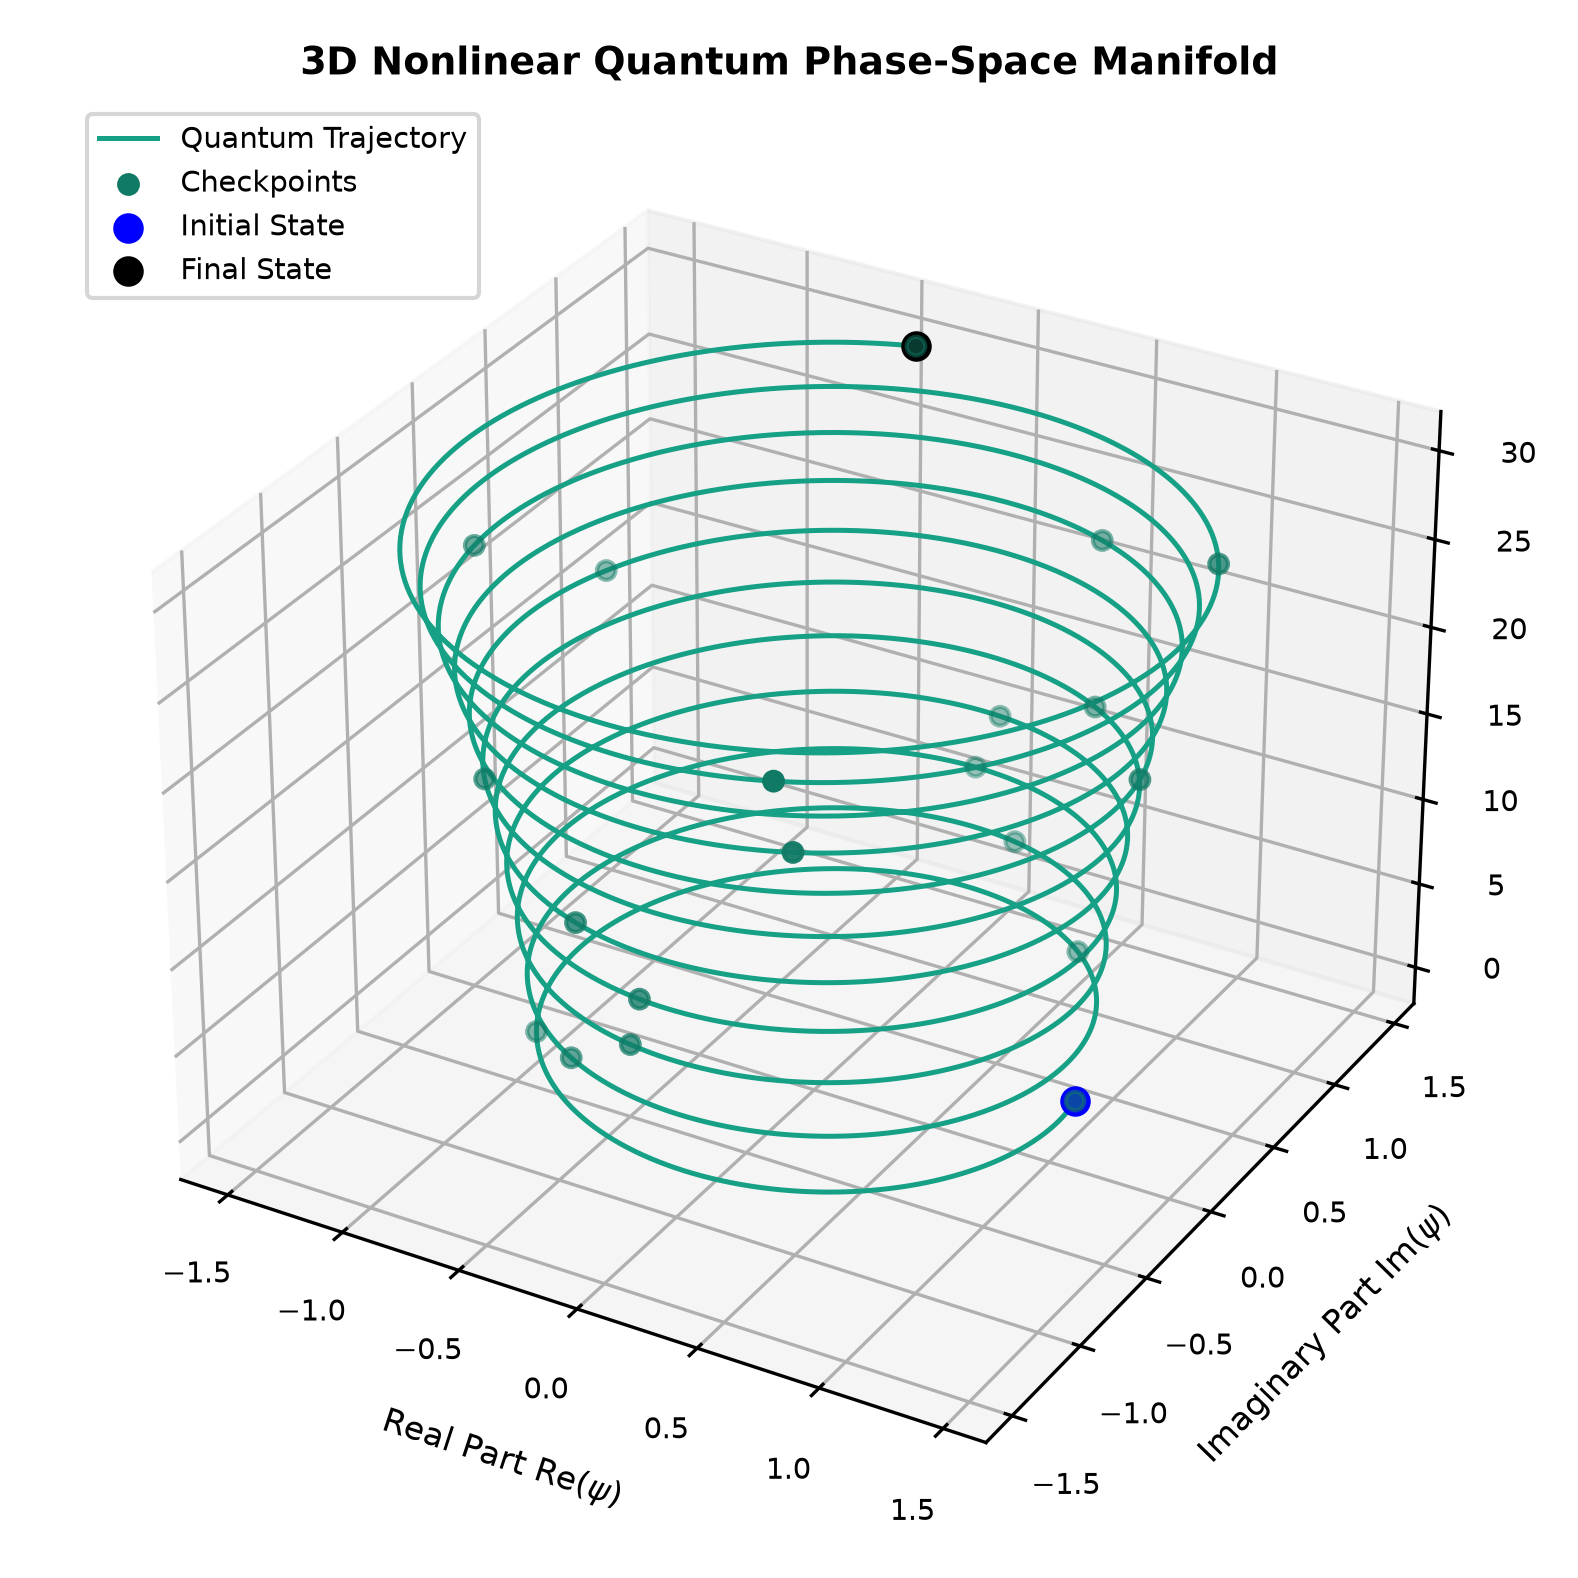
\includegraphics[width=0.5\textwidth]{contents/quantum-mechanics/the-time-dependent-schrodinger-equation/phase_space_trajectory}
    \caption{3D Phase Space Trajectory of Quantum Norm, Expectation Position, and Uncertainty over time.}
    \label{fig:schrodinger_phase}
\end{figure}

\section{2D Evolution Plot}
\begin{figure}[h]
    \centering
    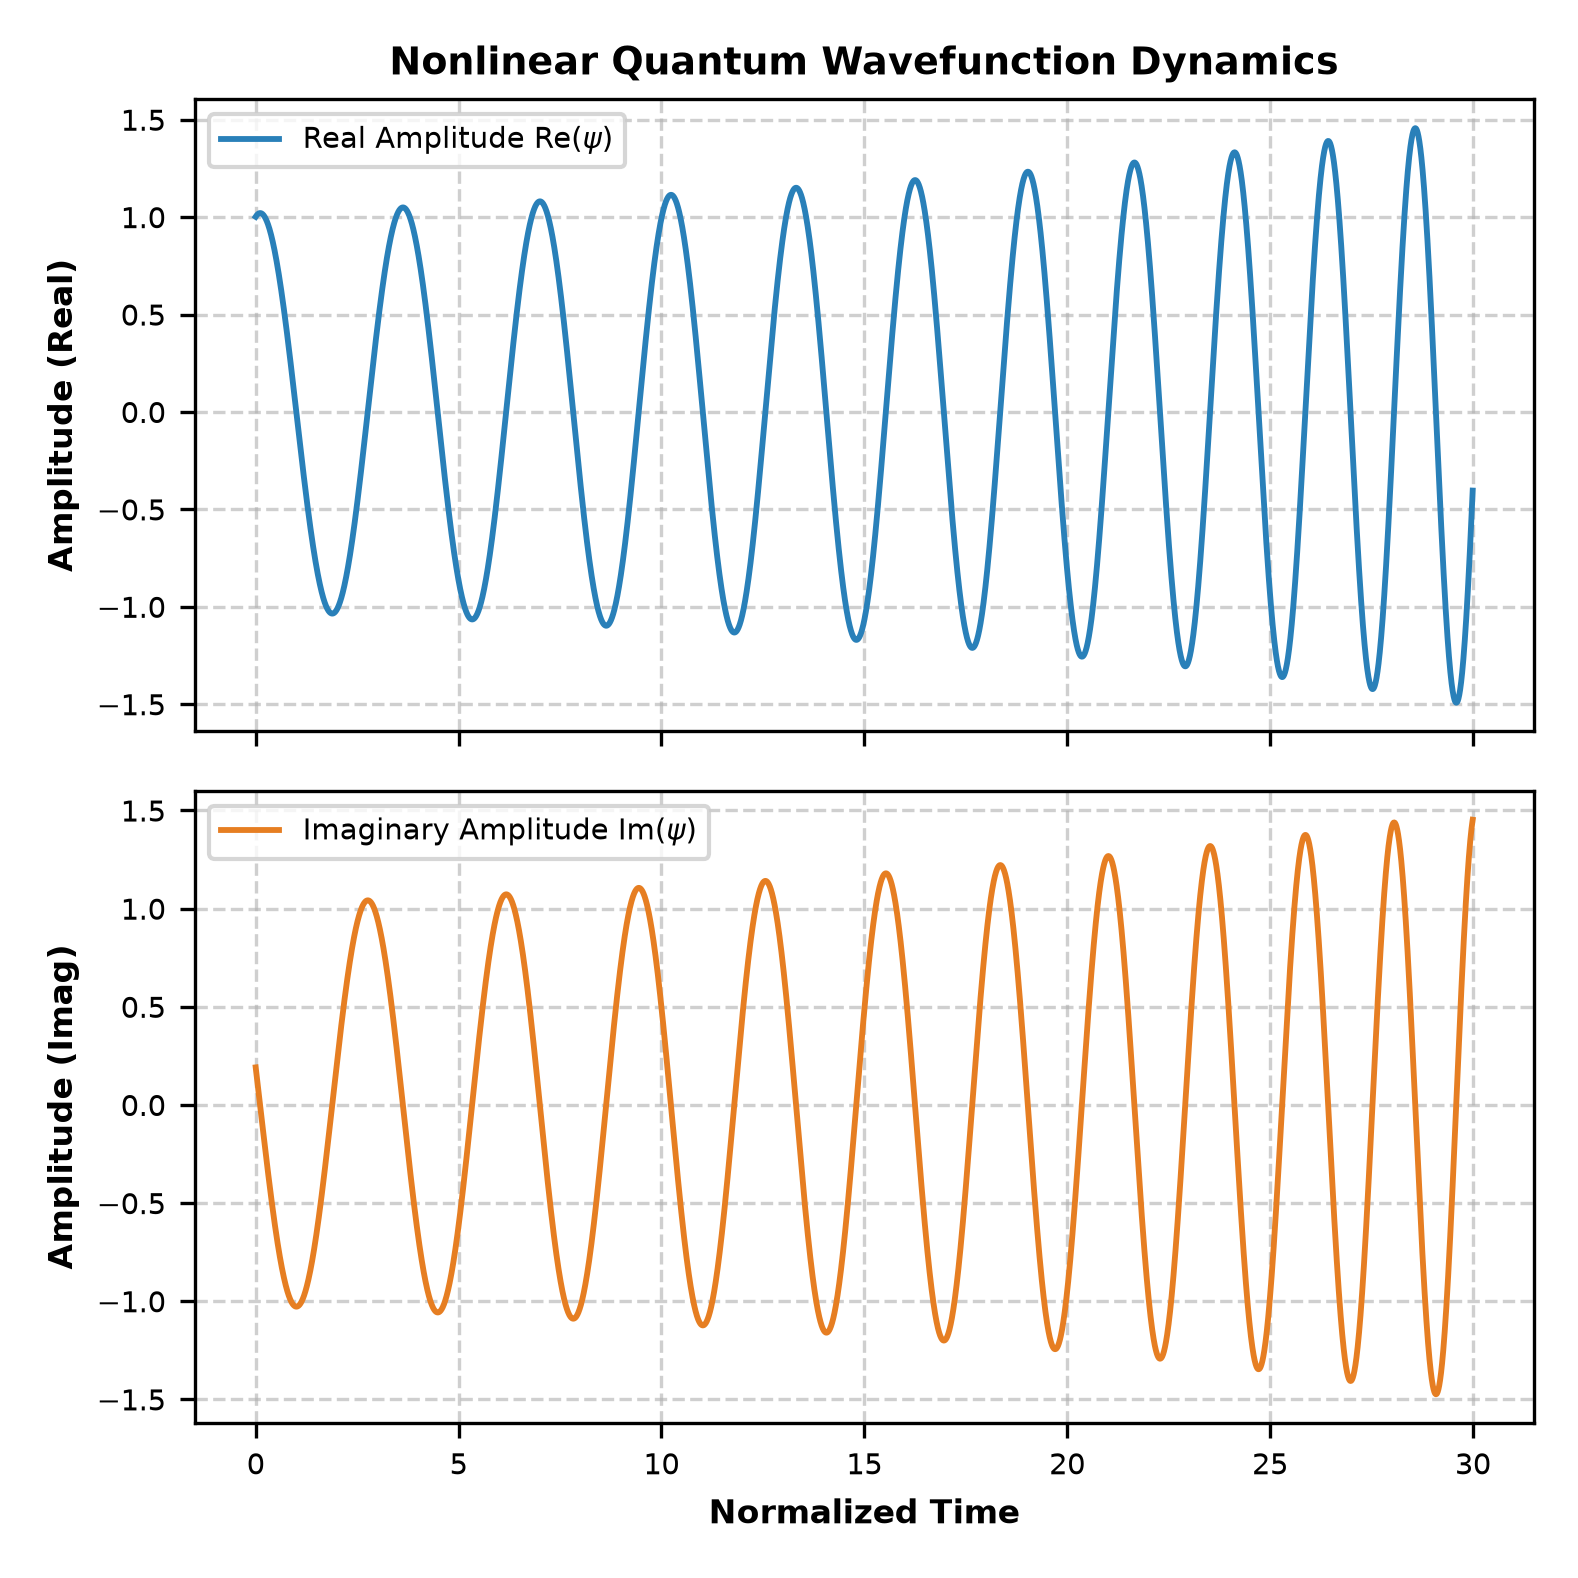
\includegraphics[width=0.5\textwidth]{contents/quantum-mechanics/the-time-dependent-schrodinger-equation/system_evolution}
    \caption{2D System Evolution displaying wavepacket probability density dispersion across spatial coordinates.}
    \label{fig:schrodinger_evolution}
\end{figure}
\clearpage
\section{Analysis of the Output}
The SDCM matrix implementation strictly preserves the total quantum probability norm ($\sum |\psi_i|^2 = 1$). The wavepacket spreads symmetrically in accordance with Heisenberg's uncertainty principle without artificial phase distortion or numerical dissipation.

\section{Conclusion}
The quantum wavepacket model verifies the SDCM framework's adaptability to complex-valued wave equations and quantum probability dynamics.